%!TeX root = main.tex
%!encoding = UTF-8 Unicode
\section{Operating-Point Study}

\subsection{Gate Resistance}

\begin{figure}[ht]
	\centering
	\begin{subfigure}[t]{\textwidth}
		\centering
		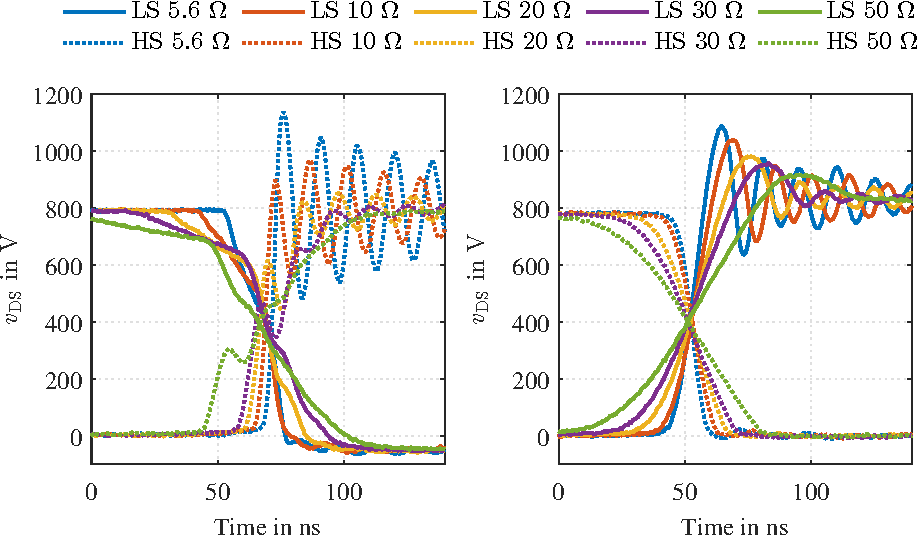
\includegraphics[scale = 1]{figures/7_MeasurementResults/MR_Rg/MR_Rg_Voltage_TD.pdf}
		\subcaption{Time-domain voltage measurement results.}
		\label{fig:MR_Rg_Sweep_Voltage_TD}
	\end{subfigure} 
    
	\vspace{0.5cm}	
	
    \begin{subfigure}[t]{\textwidth}
		\centering
		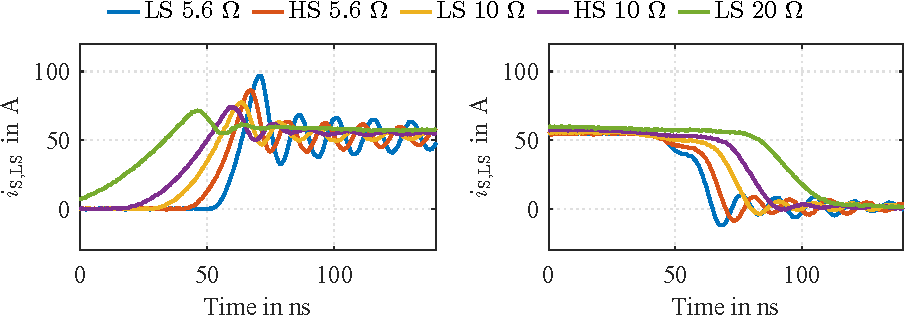
\includegraphics[scale = 1]{figures/7_MeasurementResults/MR_Rg/MR_Rg_Current_TD.pdf}
		\subcaption{Time-domain current measurement results.}
		\label{fig:MR_Rg_Sweep_Current_TD}
	\end{subfigure}
	\caption{Time-domain results of the gate-resistance sweep.}
\end{figure}

\begin{figure}[ht]
	\centering
	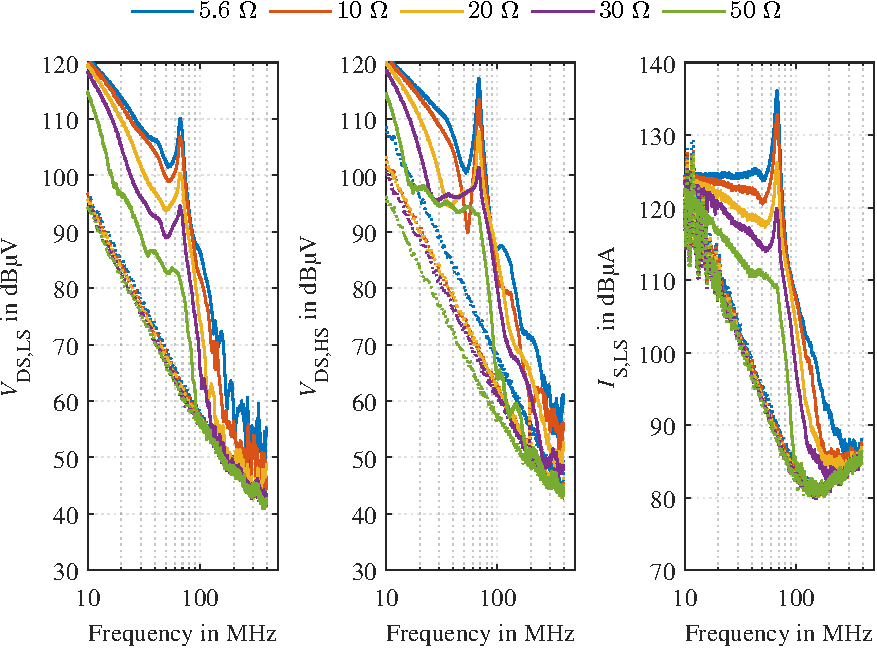
\includegraphics[scale = 1]{figures/7_MeasurementResults/MR_Rg/MR_Rg_FD.pdf}
	\caption{Frequency-domain measurement results of gate resistance sweep.}\label{fig:MR_Rg_Sweep_FD}
\end{figure}


\begin{figure}[ht]
	\centering
	\begin{subfigure}[t]{\textwidth}
		\centering
		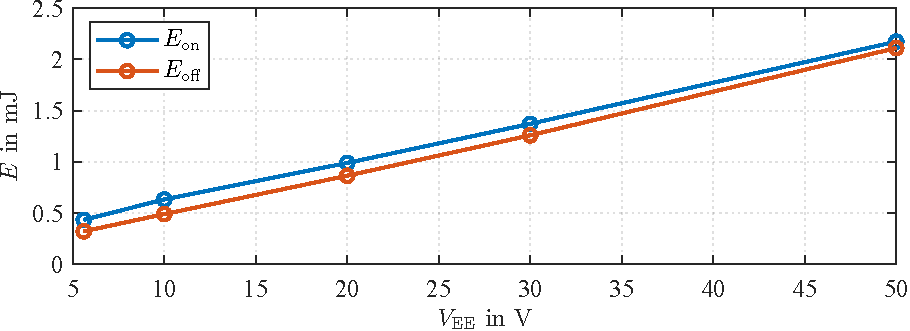
\includegraphics[scale = 1]{figures/7_MeasurementResults/MR_Rg/MR_Rg_Losses.pdf}
		\subcaption{Influence of gate resistance and switching losses on the EM emissions.}
		\label{fig:MR_Rg_EmissionOverLosses}
	\end{subfigure} 

	\vspace{0.5cm}
	
    \begin{subfigure}[t]{\textwidth}
		\centering
		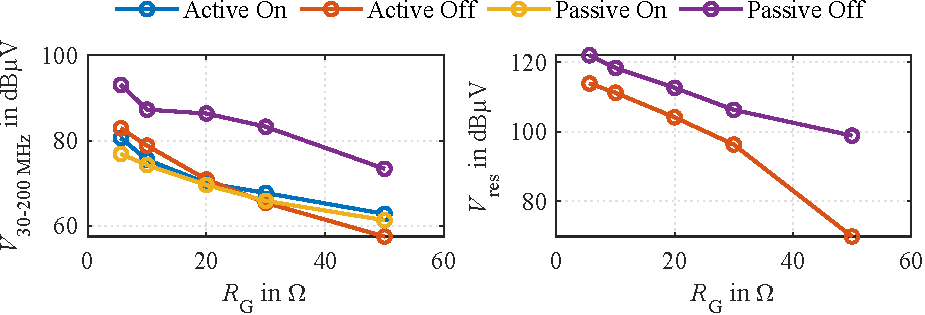
\includegraphics[scale = 1]{figures/7_MeasurementResults/MR_Rg/MR_Rg_Emission.pdf}
		\subcaption{EM emissions separated for turn-on and turn-off.}
		\label{fig:MR_Rg_Emission}
	\end{subfigure}
	\caption{Gate-resistance-dependent emission and loss analysis.}
\end{figure}


\subsection{Negative Gate-Driver Bias}



\begin{figure}[ht]
	\centering
	\begin{subfigure}[t]{\textwidth}
		\centering
		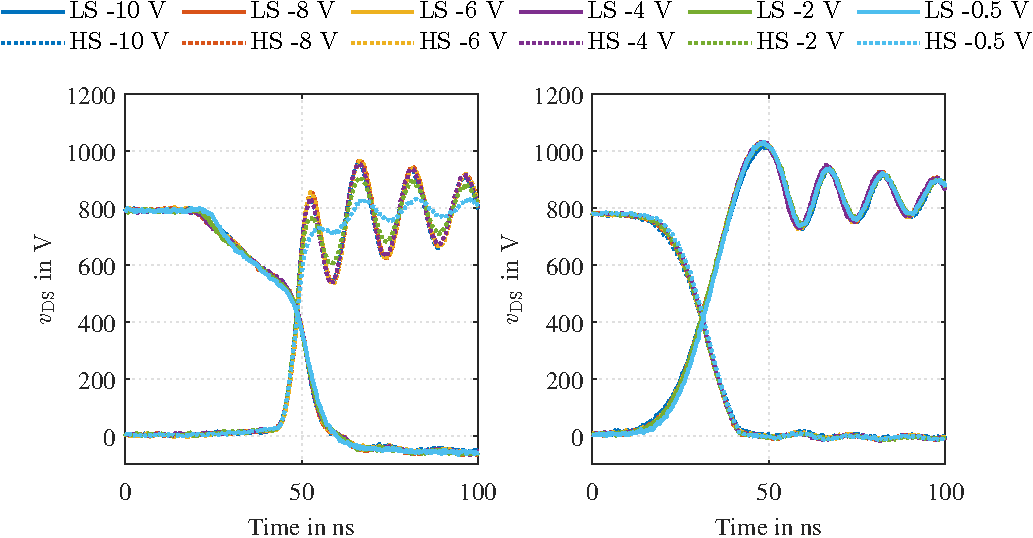
\includegraphics[scale = 1]{figures/7_MeasurementResults/MR_Vee_constE/MR_Vee_constE_Voltage_TD.pdf}
		\subcaption{Time-domain voltage measurement results.}
		\label{fig:MR_Vee_constE_Sweep_Voltage_TD}
	\end{subfigure} 
    
	\vspace{0.5cm}	
	
    \begin{subfigure}[t]{\textwidth}
		\centering
		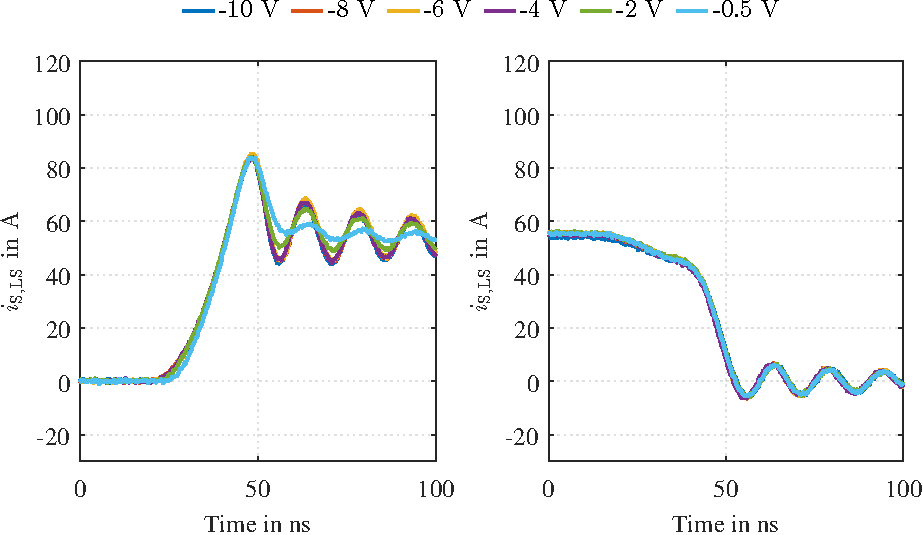
\includegraphics[scale = 1]{figures/7_MeasurementResults/MR_Vee_constE/MR_Vee_constE_Current_TD.pdf}
		\subcaption{Time-domain current measurement results.}
		\label{fig:MR_Vee_constE_Sweep_Current_TD}
	\end{subfigure}
	\caption{Time-domain results of the negative gate-driver bias sweep.}
\end{figure}

\begin{figure}[ht]
	\centering
	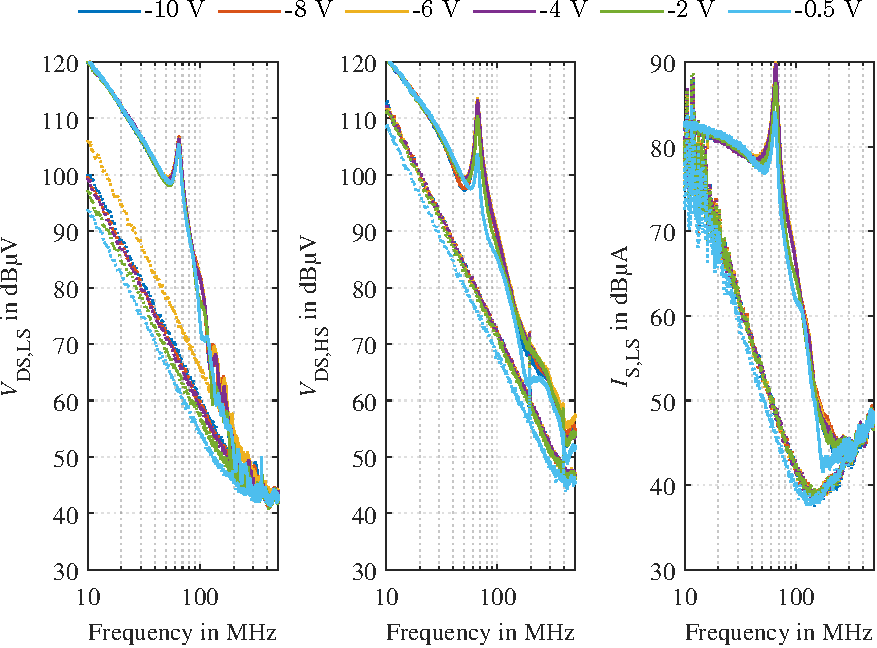
\includegraphics[scale = 1]{figures/7_MeasurementResults/MR_Vee_constE/MR_Vee_constE_FD.pdf}
	\caption{Frequency-domain measurement results of negative gate-driver bias sweep.}\label{fig:MR_Vee_constE_Sweep_FD}
\end{figure}


\begin{figure}[ht]
	\centering
	\begin{subfigure}[t]{\textwidth}
		\centering
		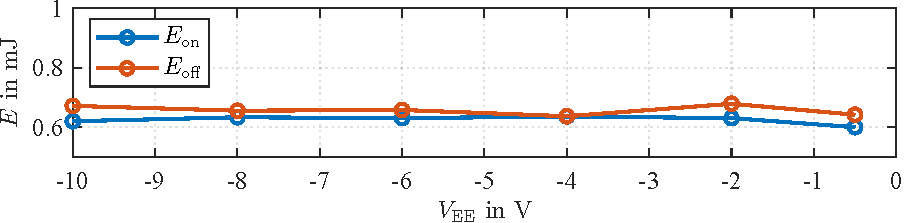
\includegraphics[scale = 1]{figures/7_MeasurementResults/MR_Vee_constE/MR_Vee_constE_Losses.pdf}
		\subcaption{Influence of negative gate-driver bias and switching losses on the EM emissions.}
		\label{fig:MR_Vee_constE_EmissionOverLosses}
	\end{subfigure} 

	\vspace{0.5cm}
	
    \begin{subfigure}[t]{\textwidth}
		\centering
		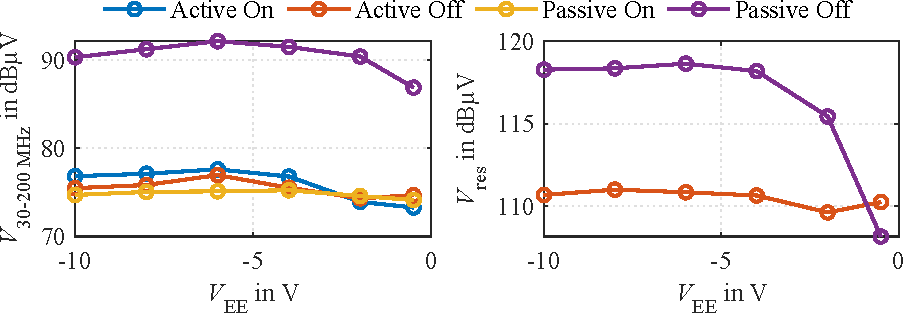
\includegraphics[scale = 1]{figures/7_MeasurementResults/MR_Vee_constE/MR_Vee_constE_Emission.pdf}
		\subcaption{EM emissions separated for turn-on and turn-off.}
		\label{fig:MR_Vee_constE_Emission}
	\end{subfigure}
	\caption{Negative gate-driver-bias-dependent emission and loss analysis.}
\end{figure}

